\documentclass[UTF8]{ctexart}
\usepackage{amsmath}
\usepackage{amssymb}
\usepackage{geometry}
\usepackage{graphicx}
\usepackage{hyperref}
\usepackage{listings}
\usepackage{tikz}
\usepackage{enumerate}

\geometry{a4paper, margin=1in}

\title{计算机图形学复习资料}
\author{Antigravity 辅助整理}
\date{\today}

\begin{document}

\maketitle
\tableofcontents

\newpage

\section{图形学基本概念}

\begin{enumerate}
    \item \textbf{什么是计算机图形学？}
    计算机图形学是研究如何用计算机生成、处理和显示图形的一门学科。它主要关注如何将数学模型转换为可见的图像。

    \item \textbf{计算机图形学的主要研究内容包括哪些？}
    \begin{itemize}
        \item \textbf{硬件部分}：输入设备、输出设备（显示器）、图形处理器（GPU）。
        \item \textbf{软件部分}：图形生成算法（如直线、圆生成）、图形变换算法（平移、旋转、缩放）、图形显示技术（消隐、渲染流水线）、建模技术。
    \end{itemize}

    \item \textbf{计算机图形学的主要应用领域。}
    主要包括：CAD/CAM（计算机辅助设计与制造）、可视化技术（医学、地理）、计算机辅助教学、娱乐（影视特效、游戏）、虚拟现实（VR）、艺术创作等。

    \item \textbf{图形和图像的主要区别是什么？}
    \begin{itemize}
        \item \textbf{图形 (Graphics)}：由基本几何体（点、线、面等）构成的实体，具有几何属性和视觉属性。它是通过算法生成的参数化表示。
        \item \textbf{图像 (Image)}：由离散的像素点构成的点阵信息。它是通过照相机等设备对真实场景的采样或由图形算法渲染后的结果。
    \end{itemize}

    \item \textbf{计算机图形处理系统的主要构成。}
    包含硬件系统（主机、显卡、显示器、交互设备）和软件系统（图形标准、图形软件开发工具、应用程序）。

    \item \textbf{显卡的工作流程。}
    数据流向：CPU $\to$ GPU $\to$ 帧缓冲器（显存） $\to$ 视频控制器 $\to$ 显示屏。
    具体步骤：
    \begin{enumerate}
        \item CPU将处理后的图形数据通过总线送入GPU。
        \item GPU处理数据并将结果存入帧缓冲器。
        \item 视频控制器从帧缓冲器读取像素信息，通过DAC（数模转换）等处理后输出。
        \item 信号驱动显示器显示图像。
    \end{enumerate}

    \item \textbf{什么是显示存储器？}
    简称显存或帧缓冲器（Frame Buffer）。它用来存储屏幕上每个像素的颜色值。显存中的存储单元与屏幕像素一一对应，其大小直接决定了屏幕的分辨率。

    \item \textbf{GPU的基本概念。}
    GPU（图形处理器）是专为执行复杂的数学和几何计算而设计的微处理器。它能够将复杂的图形转换成显示器能够显示的图像，支持大规模并行计算。

    \item \textbf{显卡分辨率的含义。}
    指显卡输出到显示器的像素点数量（如 $1920 \times 1080$）。分辨率由显存大小和视频控制器上的 RAM DAC 速率决定。如果显存足够大，则 RAM DAC 决定了分辨率的最大值。

    \item \textbf{GPU堆包含哪几种主要的类型，具有什么样的特点？}
    Direct3D 12 中将其分为：
    \begin{itemize}
        \item \textbf{上传堆 (Upload Heap)}：用于将数据从CPU传输到GPU，CPU可写。
        \item \textbf{默认堆 (Default Heap)}：GPU访问最快的堆，CPU通常不可访，适合存储频繁使用的图形资源（如纹理、顶点缓冲）。
        \item \textbf{回读堆 (Readback Heap)}：用于将数据从GPU传输回CPU。
    \end{itemize}

    \item \textbf{GPU渲染流水线包含哪几个阶段，分别完成什么任务？}
    主要阶段包括：
    \begin{itemize}
        \item \textbf{输入装配阶段}：读取顶点和索引，生成基本几何图元（点、线、三角形）。
        \item \textbf{顶点着色阶段}：完成顶点变换（如局部坐标到齐次裁剪坐标）、光照转换等。
        \item \textbf{外壳着色阶段}、\textbf{曲面细分阶段}、\textbf{域着色阶段}：用于精细化图形，将大三角形分解为小三角形。
        \item \textbf{几何着色阶段}：筛选输入的点或生成新的几何图元。
        \item \textbf{光栅化阶段}：将几何图元转换为二维图像，确定哪些栅格被占用，分配颜色和深度。
        \item \textbf{像素着色阶段}：计算每个像素的最终颜色（光照、阴影、纹理采样）。
        \item \textbf{输出融合阶段}：处理深度测试和混合，将像素合并到后台缓冲区。
    \end{itemize}
    \textbf{补充：裁剪（Clipping）}通常由硬件在光栅化前完成。

    \item \textbf{光照的基本原理}
    物体颜色由材质属性和光照环境共同决定。主要涉及光纤的反射、拆射和吸收。

    \item \textbf{光照模型的分类}
    包含局部光照模型（只考虑点状光源和物体表面）和全局光照模型（考虑光在物体间的多次反射，如光线追踪）。经典模型包括 Phong 模型。

    \item \textbf{光源的分类}
    环境光、点光源、平行光、聚光灯等。

    \item \textbf{纹理的表现形式。}
    主要表现为纹理贴图（Texture Mapping），包括一维、二维和三维纹理。

    \item \textbf{纹理的过滤方式及寻址方式}
    \begin{itemize}
        \item \textbf{过滤方式}：最近邻取样、线性过滤（双线性、三线性、各向异性过滤）。
        \item \textbf{寻址方式}：重复（Wrap）、镜像（Mirror）、夹持（Clamp）等。
    \end{itemize}

    \item \textbf{多级纹理 (Mipmapping) 的基本原理}
    为了避免在远处出现摩尔纹（采样不足），预先生成一系列分辨率递减的纹理图像，根据物体距离选择合适的层级进行采样。

    \item \textbf{模型的表示方法}
    边界表示（用表面三角形网格表示）、体素表示、参数化表示（如 Bezier 曲面）等。

    \item \textbf{Direct3D 12 图形绘制的基本原理}
    通过命令队列、命令列表管理GPU任务，利用管线状态对象 (PSO) 预处理管线配置，使用资源屏障管理同步，提高并行度和效率。

    \item \textbf{三维模型顶点的数据结构表示}
    通常包含：位置（Position）、颜色（Color）、法线（Normal）、纹理坐标（TexCoord）等。
\end{enumerate}

\section{图形学基本算法}

\subsection{直线生成算法}

\subsubsection{DDA 算法 (Digital Differential Analyzer)}
\textbf{详细原理}：DDA 算法基于直线的微分方程 $dy/dx = m$。当 $\Delta x = 1$ 时，$\Delta y = m$。
\begin{itemize}
    \item \textbf{执行过程}：
        \begin{enumerate}
            \item 计算 $dx = x_1 - x_0, dy = y_1 - y_0$。
            \item 确定步进主方向：$Length = \max(|dx|, |dy|)$。
            \item 计算增量：$\Delta x = dx/Length, \Delta y = dy/Length$。
            \item 迭代更新：$x_{i+1} = x_i + \Delta x, y_{i+1} = y_i + \Delta y$。
            \item 绘制点时对坐标四舍五入：$SetPixel(\text{int}(x+0.5), \text{int}(y+0.5))$。
        \end{enumerate}
    \item \textbf{好记口诀}：增量步进，四舍五入。
    \item \textbf{计算例题}：绘制从 $(0,0)$ 到 $(5,2)$ 的直线。
        \begin{itemize}
            \item $dx=5, dy=2, Length=5$。
            \item $\Delta x = 1, \Delta y = 0.4$。
        \end{itemize}
        \textbf{参数变化表}：
        \begin{center}
        \begin{tabular}{|c|c|c|c|}
            \hline
            步数 $i$ & $x$ & $y$ & 绘制点 $(round(x), round(y))$ \\
            \hline
            0 & 0 & 0 & (0, 0) \\
            1 & 1 & 0.4 & (1, 0) \\
            2 & 2 & 0.8 & (2, 1) \\
            3 & 3 & 1.2 & (3, 1) \\
            4 & 4 & 1.6 & (4, 2) \\
            5 & 5 & 2.0 & (5, 2) \\
            \hline
        \end{tabular}
        \end{center}
    \item \textbf{缺点}：涉及浮点加法和取整运算，在大范围绘图时会有累计误差。
    \item \textbf{变量含义与变化原因}：
    \begin{itemize}
        \item $\Delta x, \Delta y$：每一步的增量。原因：利用直线的线性性质 $y = kx + b$，当 $x$ 增加 1，$y$ 必然增加 $k$。
        \item $round(x), round(y)$：像素坐标。原因：屏幕栅格是离散的整数网格，必须将浮点坐标映射到最近的整数点。
    \end{itemize}
    \item \textbf{示意图}：
    \begin{center}
    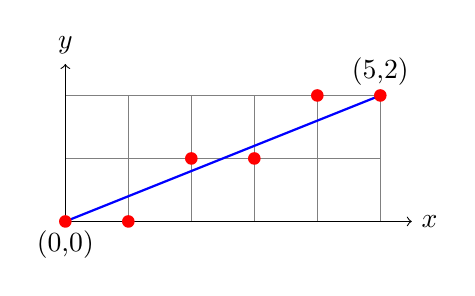
\begin{tikzpicture}[scale=0.8]
        \draw[help lines] (0,0) grid (5,2);
        \draw[->] (0,0) -- (5.5,0) node[right] {$x$};
        \draw[->] (0,0) -- (0,2.5) node[above] {$y$};
        \draw[thick, blue] (0,0) -- (5,2);
        \foreach \x/\y in {0/0, 1/0, 2/1, 3/1, 4/2, 5/2}
            \fill[red] (\x,\y) circle (0.1);
        \node[below] at (0,0) {(0,0)};
        \node[above] at (5,2) {(5,2)};
    \end{tikzpicture}
    \end{center}
\end{itemize}

\subsubsection{中点画线法}
\textbf{详细推导}：
设直线方程为 $F(x,y) = ax + by + c = 0$，其中 $a = y_0 - y_1, b = x_1 - x_0, c = x_0 y_1 - x_1 y_0$。
对于 $0 < m < 1$，当前点为 $(x_i, y_i)$，下一个点可能是 $P_1(x_i+1, y_i)$ 或 $P_2(x_i+1, y_i+1)$。
\begin{itemize}
    \item \textbf{判别式}：$d = F(x_i+1, y_i+0.5)$。
    \item \textbf{增量推导}：
        \begin{itemize}
            \item 若 $d \ge 0$ (中点在直线上方或直线上)，选下方的点 $P_1$。下一步判别式 $d_{new} = F(x_i+2, y_i+0.5) = d + a$。增量为 $a$。
            \item 若 $d < 0$ (中点在直线下方)，选上方的点 $P_2$。下一步判别式 $d_{new} = F(x_i+2, y_i+1.5) = d + a + b$。增量为 $a + b$。
        \end{itemize}
    \item \textbf{初始值}：$d_0 = F(x_0+1, y_0+0.5) = a + 0.5b$。通常使用 $2d_0 = 2a + b$ 消除浮点。
    \item \textbf{计算例题}：绘制从 $(0,0)$ 到 $(5,2)$ 的直线。
        \begin{itemize}
            \item $a = 0-2 = -2$; $b = 5-0 = 5$。
            \item $d_0 = 2a + b = 2(-2) + 5 = 1$。
            \item $\Delta d_1 = 2a = -4$ (当 $d \ge 0$); $\Delta d_2 = 2(a+b) = 6$ (当 $d < 0$)。
        \end{itemize}
        \textbf{参数变化表}：
        \begin{center}
        \begin{tabular}{|c|c|c|c|c|}
            \hline
            步数 $i$ & $d$ & 选择点 & 下一步 $d$ 更新 & 绘制点 \\
            \hline
            0 & 1 & $P_1$ & $1+(-4)=-3$ & (0,0) \\
            1 & -3 & $P_2$ & $-3+6=3$ & (1,0) \\
            2 & 3 & $P_1$ & $3+(-4)=-1$ & (2,1) \\
            3 & -1 & $P_2$ & $-1+6=5$ & (3,1) \\
            4 & 5 & $P_1$ & $5+(-4)=1$ & (4,2) \\
            5 & 1 & - & - & (5,2) \\
            \hline
        \end{tabular}
        \end{center}
    \item \textbf{变量含义与变化原因}：
    \begin{itemize}
        \item $F(x,y)$：隐式直线方程。含义：点 $(x,y)$ 到直线的代数距离(未归一化)。
        \item $d$：判别式。含义：中点 $M(x_i+1, y_i+0.5)$ 的函数值 $F(M)$。
        \item \textbf{变化原因}：
            \begin{itemize}
                \item 若 $d \ge 0$，$M$ 在直线上方，说明交点在 $M$ 下方，应取 $P_1(x_i+1, y_i)$，离直线更近。
                \item 若 $d < 0$，$M$ 在直线下方，说明交点在 $M$ 上方，应取 $P_2(x_i+1, y_i+1)$。
            \end{itemize}
    \end{itemize}
    \item \textbf{示意图}：
    \begin{center}
    \begin{tikzpicture}[scale=1]
        \draw[help lines] (0,0) grid (3,2);
        \draw[thick, blue] (0,0.2) -- (3,1.8);
        
        \fill[black] (1,0) circle (0.1) node[below] {$(x_i, y_i)$};
        \fill[gray] (2,0) circle (0.05) node[below right] {$P_1$};
        \fill[gray] (2,1) circle (0.05) node[above right] {$P_2$};
        \fill[red] (2,0.5) circle (0.05) node[right] {$M$};
        
        \node at (2.5, 1.5) {直线在$M$上方 $\Rightarrow d<0$};
    \end{tikzpicture}
    \end{center}
\end{itemize}

\subsubsection{Bresenham 算法 (全象限推广)}
\textbf{核心逻辑}：
Bresenham 算法通过整数误差项 $d$ 来控制是否在垂直主位移方向进位。
\begin{itemize}
    \item \textbf{执行步骤 (以第一象限 $0 < m < 1$ 为例)}：
        \begin{enumerate}
            \item $d = 2\Delta y - \Delta x$。
            \item \textbf{更新逻辑}：
                \begin{itemize}
                    \item 若 $d < 0$：$d = d + 2\Delta y, x = x + 1$。
                    \item 若 $d \ge 0$：$d = d + 2(\Delta y - \Delta x), x = x + 1, y = y + 1$。
                \end{itemize}
        \end{enumerate}
    \item \textbf{计算例题}：绘制从 $(0,0)$ 到 $(5,2)$ 的直线。
        \begin{itemize}
            \item $\Delta x = 5, \Delta y = 2$。
            \item $d_0 = 2\Delta y - \Delta x = 4 - 5 = -1$。
        \end{itemize}
        \textbf{参数变化表}：
        \begin{center}
        \begin{tabular}{|c|c|c|c|}
            \hline
            步数 $i$ & $d$ & $y$ 变化 & 绘制点 $(x, y)$ \\
            \hline
            0 & -1 & 不变 & (0, 0) \\
            1 & $-1+4=3$ & 进位 & (1, 0) \\
            2 & $3+2(2-5)=-3$ & 不变 & (2, 1) \\
            3 & $-3+4=1$ & 进位 & (3, 1) \\
            4 & $1+2(2-5)=-5$ & 不变 & (4, 2) \\
            5 & - & - & (5, 2) \\
            \hline
        \end{tabular}
        \end{center}
    \item \textbf{推广到全局 8 个区域 (所有情况)}：
        根据斜率 $k$ 和端点相对位置，将线段归类为 8 个区域。
        \begin{itemize}
            \item \textbf{处理逻辑}：
                \begin{itemize}
                    \item 若 $|dx| < |dy|$（区域 2, 3, 6, 7）：交换 $x$ 和 $y$ 坐标计算，绘制时再交换回来。
                    \item 若 $x_0 > x_1$（区域 3, 4, 5, 6）：通过交换起点和终点，变换到 $y$ 轴右侧区域（区域 7, 8, 1, 2）。
                    \item 若斜率 $k < 0$（区域 7, 8）：对 $y$ 轴做镜像变换，计算完后再镜像回来。
                \end{itemize}
        \end{itemize}
    \item \textbf{好记口诀}：\textbf{主轴步进累加，误差偏离进位。}
\end{itemize}

\textbf{C++ 实现片段 (支持全象限处理思路)}:
\begin{lstlisting}[language=C++]
void BresenhamLine(int x0, int y0, int x1, int y1) {
    int dx = abs(x1 - x0), dy = abs(y1 - y0);
    int sx = x0 < x1 ? 1 : -1, sy = y0 < y1 ? 1 : -1;
    int err = dx - dy, e2;
    while (true) {
        SetPixel(x0, y0);
        if (x0 == x1 && y0 == y1) break;
        e2 = 2 * err;
        if (e2 > -dy) { err -= dy; x0 += sx; }
        if (e2 <  dx) { err += dx; y0 += sy; }
    }
}
\end{lstlisting}

\subsection{圆和圆弧生成算法}

\subsubsection{中点画圆法 (Midpoint Circle Algorithm)}
\textbf{核心思想}：利用圆的八对称性。只需计算 $0^\circ \sim 45^\circ$（$x=0$ 到 $x=y$）的弧段。
$f(x,y) = x^2 + y^2 - R^2 = 0$。
\begin{itemize}
    \item \textbf{判别式推导}：$d = f(x_i+1, y_i-0.5)$。
    \item \textbf{更新策略}：
        \begin{itemize}
            \item $d < 0$：取点 $(x_i+1, y_i)$，更新 $d = d + 2x_i + 3$。
            \item $d \ge 0$：取点 $(x_i+1, y_i-1)$，更新 $d = d + 2(x_i - y_i) + 5$。
        \end{itemize}
    \item \textbf{初始值}：$d = 1.25 - R$ (整数取 $1-R$)。
    \item \textbf{计算例题}：半径 $R=10$ 的第一八分圆。
        \begin{center}
        \begin{tabular}{|c|c|c|c|c|}
            \hline
            步数 $n$ & $d$ & 选择点 & 下一步 $d$ & 绘制点 $(x, y)$ \\
            \hline
            0 & -9 & $d < 0$ & $-9+2(0)+3=-6$ & (0, 10) \\
            1 & -6 & $d < 0$ & $-6+2(1)+3=-1$ & (1, 10) \\
            2 & -1 & $d < 0$ & $-1+2(2)+3=6$ & (2, 10) \\
            3 & 6 & $d \ge 0$ & $6+2(3-10)+5=-5$ & (3, 10) \\
            4 & -5 & $d < 0$ & $-5+2(4)+3=6$ & (4, 9) \\
            5 & 6 & $d \ge 0$ & $6+2(5-9)+5=3$ & (5, 9) \\
            6 & 3 & $d \ge 0$ & $3+2(6-8)+5=4$ & (6, 8) \\
            7 & 4 & 停止 ($x > y$) & - & (7, 7) \\
            \hline
        \end{tabular}
        \end{center}
\end{itemize}

\subsubsection{Bresenham 画圆算法}
\textbf{详细原理}：
该算法旨在寻找最接近理想圆弧的整数像素点。与中点法不同，Bresenham 算法不仅仅判断中点，而是根据误差的符号动态选择三个可能的候选点：右方($H$)、右下方($D$)、下方($V$)。
\begin{itemize}
    \item \textbf{误差函数}：定义 $D(x,y) = |(x^2 + y^2) - R^2|$ 为点到圆心的距离平方差的绝对值。算法的目标是使每一步选择的点让误差最小。
    \item \textbf{判别式递推} (第一象限 $0 \le x \le y$)：
        \begin{enumerate}
            \item \textbf{初始误差}：$\Delta = 2(1-R)$。
            \item \textbf{走向判断规则}：
                \begin{itemize}
                    \item 若 $\Delta < 0$ (当前点在圆内)：
                        \begin{itemize}
                            \item 计算 $\delta = 2(\Delta + y) - 1$。
                            \item 若 $\delta \le 0$，取右方点 $H(x+1, y)$。更新 $\Delta = \Delta + 2x + 1$。
                            \item 若 $\delta > 0$，取右下方点 $D(x+1, y-1)$。更新 $\Delta = \Delta + 2x - 2y + 2$。
                        \end{itemize}
                    \item 若 $\Delta > 0$ (当前点在圆外)：
                        \begin{itemize}
                            \item 计算 $\delta = 2(\Delta - x) - 1$。
                            \item 若 $\delta \le 0$，取右下方点 $D(x+1, y-1)$。更新 $\Delta = \Delta + 2x - 2y + 2$。
                            \item 若 $\delta > 0$，取下方点 $V(x, y-1)$。更新 $\Delta = \Delta - 2y + 1$。
                        \end{itemize}
                    \item 若 $\Delta = 0$ (正好在圆上)：直取右下方点 $D$。
                \end{itemize}
        \end{enumerate}
    \item \textbf{变量含义与变化原因}：
    \begin{itemize}
        \item $\Delta$：距离平方差。含义：当前点距离理想圆弧的“偏移量”。
        \item $\delta$：辅助判别式。含义：用于在 $\Delta < 0$ 时比较 $H$ 和 $D$ 哪个更近，或在 $\Delta > 0$ 时比较 $D$ 和 $V$ 哪个更近。
        \item \textbf{变化原因}：
            \begin{itemize}
                \item 当 $\Delta < 0$ 时，点在圆内，只能向外走（右或右下）。$\delta$ 实际上比较了 $|H^2-R^2|$ 和 $|D^2-R^2|$ 的大小。
                \item 当 $\Delta > 0$ 时，点在圆外，只能向内走（右下或下）。
            \end{itemize}
    \end{itemize}
    \item \textbf{示意图 (候选点选择)}：
    \begin{center}
    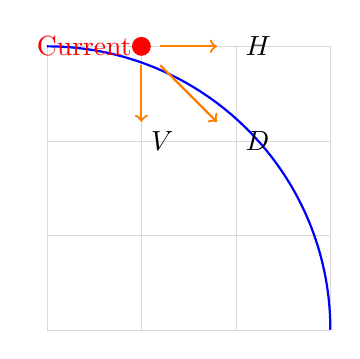
\begin{tikzpicture}[scale=1.2]
        \draw[step=1,gray!30,very thin] (0,0) grid (3,3);
        \draw[thick, blue] (0,3) arc (90:0:3);
        \fill[red] (1,3) circle (0.1) node[left] {Current};
        
        \node[right] at (2,3) {$H$};
        \node[right] at (2,2) {$D$};
        \node[right] at (1,2) {$V$};
        
        \draw[->, orange, thick] (1.2,3) -- (1.8,3);
        \draw[->, orange, thick] (1.2,2.8) -- (1.8,2.2);
        \draw[->, orange, thick] (1,2.8) -- (1,2.2);
    \end{tikzpicture}
    \end{center}
\end{itemize}

\subsubsection{圆的八对称性 (各情况映射)}
若已算出弧段上的点 $(x, y)$，通过简单变号和交换可得其余 7 个对称点：
$(x, y), (y, x), (y, -x), (x, -y), (-x, -y), (-y, -x), (-y, x), (-x, y)$。
\textbf{意义}：计算量减少为原来的 $1/8$。
\subsection{区域填充算法}

\subsubsection{扫描线填色算法 (Scanline Fill)}
\textbf{详细原理}：按行扫描，利用多边形在扫描线方向的连贯性。
\begin{itemize}
    \item \textbf{关键数据结构}：
        \begin{itemize}
            \item \textbf{边表 (Edge Table, ET)}：形象化比喻为“\textbf{备选边库}”。按 $y_{min}$ 对边进行桶分类。每条边记录：$y_{max}$、$x_{min}$、$\Delta x$ (斜率倒数)。
            \item \textbf{活动边表 (Active Edge Table, AET)}：形象化比喻为“\textbf{当前活跃窗口}”。记录当前扫描线相交的所有边，并按 $x$ 坐标升序排列。
        \end{itemize}
    \item \textbf{特殊情况处理 (边界与顶点)}：
        \begin{itemize}
            \item \textbf{奇增偶减原则}：若扫描线穿过多边形顶点，仅当下端点位于该扫描线上时计数。或采用“下闭上开”原则。
            \item \textbf{共享边处理}：为了防止重复绘制，通常规定左闭右开、下闭上开。
        \end{itemize}
    \item \textbf{好记方法}：\textbf{ET 挑边入 AET，AET 排序定区间。}
\end{itemize}

\subsubsection{种子填充法 (Seed Fill)}
\textbf{基本思想}：从给定的种子点开始，递归或迭代地对相邻像素进行填充。
\textbf{分类}：
\begin{itemize}
    \item \textbf{四连通}：仅考虑上下左右。如果边界是斜的，可能会漏填。
    \item \textbf{八连通}：考虑上下左右及对角线。能处理更复杂的边界。
\end{itemize}
\textbf{算法步骤}：
\begin{enumerate}
    \item 种子像素入栈。
    \item 栈非空时：像素出栈 $\to$ 着色 $\to$ 邻域符合条件像素入栈。
\end{enumerate}

\subsection{反走样技术}
\begin{itemize}
    \item \textbf{像素细分技术}：将像素划分为子像素进行采样后再平均。
    \item \textbf{Bresenham 反走样 (区域反走样)}：根据像素与图形重叠的面积调整灰度（亮度）。
\end{itemize}

\subsection{曲线生成}

\subsubsection{Bezier 曲线}
\textbf{定义}：$P(t) = \sum_{i=0}^n P_i B_{i,n}(t)$，其中 $B_{i,n}(t)$ 是 Bernstein 基函数。
\textbf{性质}：起点过 $P_0$，终点过 $P_n$；切线方向与特征多边形首末边一致；具有凸包性。
\textbf{de Casteljau 算法}：通过递归线性插值的方法计算曲线上任意一点。
\textbf{计算例题}：已知控制点 $P_0(0,0), P_1(2,4), P_2(4,0)$，计算 $t=0.5$ 处的点。
    \textbf{递推参数表}：
    \begin{center}
    \begin{tabular}{|c|c|c|c|}
        \hline
        层级 $r$ & 计算公式 & 结果点 & 坐标 \\
        \hline
        0 & 原始控制点 & $P_0^0, P_1^0, P_2^0$ & (0,0), (2,4), (4,0) \\
        1 & $P_i^1 = (1-t)P_i^0 + tP_{i+1}^0$ & $P_0^1, P_1^1$ & (1,2), (3,2) \\
        2 & $P_0^2 = (1-t)P_0^1 + tP_1^1$ & $P_0^2$ & (2,2) \\
        \hline
    \end{tabular}
    \end{center}
    最终曲线上的点为 (2, 2)。
    \begin{itemize}
    \item \textbf{变量含义与变化原因}：
    \begin{itemize}
        \item $t$：插值参数。含义：当前点在控制点连线上的比例位置。
        \item $P_i^r$：第 $r$ 级递推点。含义：上一级两点的线性插值结果。
    \end{itemize}
    \item \textbf{示意图 (de Casteljau 构造)}：
    \begin{center}
    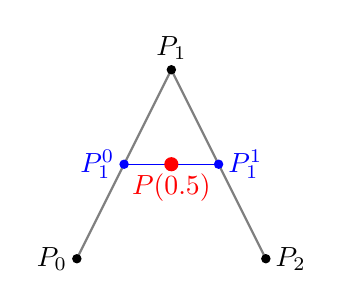
\begin{tikzpicture}[scale=0.6]
        \coordinate (P0) at (0,0);
        \coordinate (P1) at (2,4);
        \coordinate (P2) at (4,0);
        \draw[thick, gray] (P0) -- (P1) -- (P2);
        \fill (P0) circle (0.1) node[left] {$P_0$};
        \fill (P1) circle (0.1) node[above] {$P_1$};
        \fill (P2) circle (0.1) node[right] {$P_2$};
        
        \coordinate (Q0) at (1,2); % Midpoint of P0-P1
        \coordinate (Q1) at (3,2); % Midpoint of P1-P2
        \draw[blue] (Q0) -- (Q1);
        \fill[blue] (Q0) circle (0.1) node[left] {$P_1^0$};
        \fill[blue] (Q1) circle (0.1) node[right] {$P_1^1$};
        
        \coordinate (R) at (2,2); % Midpoint of Q0-Q1
        \fill[red] (R) circle (0.15) node[below] {$P(0.5)$};
    \end{tikzpicture}
    \end{center}
    \end{itemize}

\subsubsection{B 样条曲线}
\textbf{优点}：支持局部控制（修改单个点不影响全线），阶数与控制点数无关。
\textbf{基函数}：由 B-Spline 基函数定义，支持 $C^2$ 连续。

\subsection{图形变换}
\begin{itemize}
    \item \textbf{齐次坐标}：引入 $w$ 分量（通常为 1），使得平移变换可以通过 $4\times4$ 矩阵乘法实现。
    \item \textbf{常用三维变换矩阵}：
    \begin{itemize}
        \item \textbf{平移}：$T(t_x, t_y, t_z) = \begin{bmatrix} 1&0&0&t_x \\ 0&1&0&t_y \\ 0&0&1&t_z \\ 0&0&0&1 \end{bmatrix}$ (列向量表示)。
        \item \textbf{绕 X 轴旋转}：$R_x(\theta) = \begin{bmatrix} 1&0&0&0 \\ 0&\cos\theta&-\sin\theta&0 \\ 0&\sin\theta&\cos\theta&0 \\ 0&0&0&1 \end{bmatrix}$。
        \item \textbf{绕 Y 轴旋转}：$R_y(\theta) = \begin{bmatrix} \cos\theta&0&\sin\theta&0 \\ 0&1&0&0 \\ -\sin\theta&0&\cos\theta&0 \\ 0&0&0&1 \end{bmatrix}$。
        \item \textbf{绕 Z 轴旋转}：$R_z(\theta) = \begin{bmatrix} \cos\theta&-\sin\theta&0&0 \\ \sin\theta&\cos\theta&0&0 \\ 0&0&1&0 \\ 0&0&0&1 \end{bmatrix}$。
    \end{itemize}
    \item \textbf{复合变换}：矩阵乘法不满足交换律，变换顺序（如先缩放、再旋转、最后平移）对结果至关重要。
\end{itemize}

\subsection{裁剪算法}

\subsubsection{Cohen-Sutherland 算法 (所有情况分析)}
\textbf{编码规则}：$D_3 D_2 D_1 D_0$ (上、下、右、左)。
\textbf{逻辑全分支判断}：
\begin{itemize}
    \item \textbf{全取 (Inside)}：$Code1 | Code2 == 0$。两端点都在窗口内。
    \item \textbf{全弃 (Outside)}：$Code1 \& Code2 \ne 0$。两端点都在边界同一侧外。
    \item \textbf{复合情况}：线段穿过边界。选择一个在外的端点，计算其与边界的交点，用交点替换该端点后重新迭代。
\end{itemize}
\textbf{计算例题}：窗口 $W_{xmin}=0, W_{xmax}=5, W_{ymin}=0, W_{ymax}=5$。线段 $P_1(-1, 5), P_2(6, -2)$。
    \textbf{检测表格}：
    \begin{center}
    \begin{tabular}{|c|c|c|c|}
        \hline
        端点 & 坐标 & 编码 (UDRL) & 状态判断 \\
        \hline
        $P_1$ & (-1, 5) & 0001 (左) & 在左侧外 \\
        $P_2$ & (6, -2) & 0110 (下右) & 在右下外 \\
        \hline
        \multicolumn{4}{|c|}{$Code1 | Code2 = 0111 \ne 0$ (不简取), $Code1 \& Code2 = 0000 = 0$ (不简弃)} \\
        \hline
    \end{tabular}
    \end{center}
\textbf{好记方法}：\textbf{全取或运算，全弃与运算，其余切一刀。}
    \begin{itemize}
    \item \textbf{变量含义与变化原因}：
    \begin{itemize}
        \item 区域码 (Region Code)：4位二进制。含义：相对窗口的位置(上、下、右、左)。
        \item \textbf{变化原因}：通过位运算快速判断点与窗口的关系，避免昂贵的交点计算。
    \end{itemize}
    \item \textbf{示意图 (9区域编码)}：
    \begin{center}
    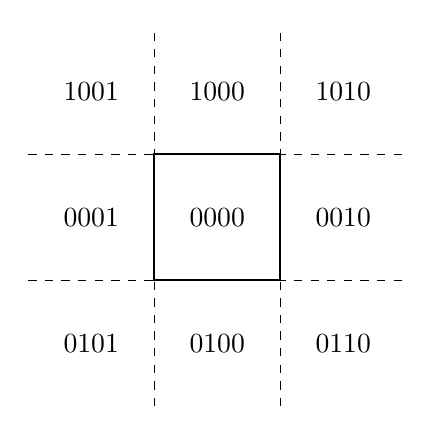
\begin{tikzpicture}[scale=0.8]
        \draw[thick] (0,0) rectangle (2,2);
        \node at (1,1) {0000};
        \node at (-1,1) {0001}; \node at (3,1) {0010};
        \node at (1,3) {1000}; \node at (1,-1) {0100};
        \node at (-1,3) {1001}; \node at (3,3) {1010};
        \node at (-1,-1) {0101}; \node at (3,-1) {0110};
        \draw[dashed] (-2,0) -- (4,0); \draw[dashed] (-2,2) -- (4,2);
        \draw[dashed] (0,-2) -- (0,4); \draw[dashed] (2,-2) -- (2,4);
    \end{tikzpicture}
    \end{center}
    \end{itemize}

\subsubsection{Liang-Barsky 算法 (特殊情况)}
\textbf{原理}：基于参数方程 $P(u) = P_1 + u(P_2 - P_1)$。
\textbf{全情况分析}：
\begin{itemize}
    \item $p_k = 0$：线段平行于第 $k$ 条边界。
        \begin{itemize}
            \item 若 $q_k < 0$，线段完全在窗外，直接舍弃。
            \item 若 $q_k \ge 0$，线段在边界内侧，继续判断其他边。
        \end{itemize}
    \item $p_k < 0$：线段由外向内。更新 $u_1 = \max(u_1, q_k/p_k)$。
    \item $p_k > 0$：线段由内向外。更新 $u_2 = \min(u_2, q_k/p_k)$。
    \item \textbf{变量含义与变化原因}：
    \begin{itemize}
        \item $u$：参数。含义：线段上点的相对位置，$u \in [0,1]$。
        \item $p_k, q_k$：几何参数。含义：$p_k$代表线段在某个方向的投影长度，$q_k$代表起点到边界的距离。
        \item \textbf{变化原因}：
            \begin{itemize}
                \item $p_k < 0$：线段从外部进入内部(入边)，应推迟起点(取 $\max$)。
                \item $p_k > 0$：线段从内部离开外部(出边)，应提前终点(取 $\min$)。
            \end{itemize}
    \end{itemize}
    \item \textbf{示意图 (参数 $u$ 更新)}：
    \begin{center}
    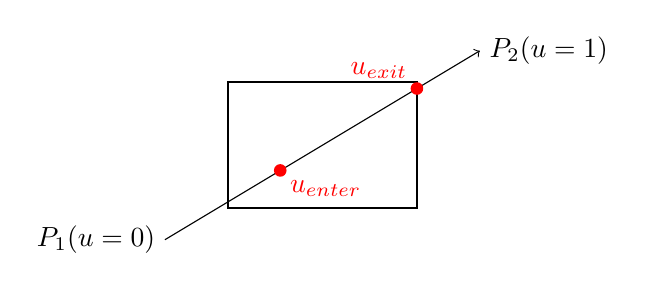
\begin{tikzpicture}[scale=0.8]
        \draw[thick] (0,0) rectangle (3,2);
        \draw[->] (-1, -0.5) node[left]{$P_1(u=0)$} -- (4, 2.5) node[right]{$P_2(u=1)$};
        \fill[red] (0.83, 0.6) circle (0.1) node[below right] {$u_{enter}$};
        \fill[red] (3, 1.9) circle (0.1) node[above left] {$u_{exit}$};
    \end{tikzpicture}
    \end{center}
\end{itemize}

\subsubsection{Sutherland-Hodgman 多边形裁剪 (4 种规则)}
\textbf{核心}：依次用四个边界裁剪多边形，输出满足条件的顶点。
\textbf{四种顶点处理规则}：
\begin{enumerate}
    \item \textbf{由内向内}：输出当前点。
    \item \textbf{由内向外}：输出交点。
    \item \textbf{由外向内}：输出交点和当前点。
    \item \textbf{由外向外}：不输出。
\end{enumerate}
\textbf{好记比喻}：\textbf{进门全带走，出门留坐标，门外不参与。}

\subsection{图形消隐}
\begin{itemize}
    \item \textbf{背面剔除}：根据面法向量与视向量的点积判断，若 $\cos\theta < 0$ 则为背面。
    \item \textbf{画家算法}：依深度从远到近绘制。
    \item \textbf{深度缓冲区 (Z-Buffer)}：每个像素保存当前最近的 $Z$ 值，比较后决定是否更新颜色。
\end{itemize}

\subsection{高级模拟}
\begin{itemize}
    \item \textbf{地形生成}：Diamond-Square 算法，通过递归中点位移产生分形地形。
    \item \textbf{雨雪模拟}：粒子系统，维护每个粒子的生命周期、位置、速度，赋予纹理。
\end{itemize}

\end{document}
